\chapter{ならし解析 - Amortized analysis}

\index{amortized analysis}

多くのプログラムにおいて、時間計算量は、アルゴリズムの構造を調べるだけで簡単に解析できます。
例えば何回ループが実行されるかといった解析を行います。
ですが、直感的な解析だけでは計算量を正しく見積もれないこともあります。

\key{ならし解析 - Amortized analysis} を使って、時間計算量が一定に定まらないような計算量を見積もることができます。
基本的なアイデアは、個々の操作に注目するのではなく、アルゴリズムの実行中に全ての操作に使用される操作の合計時間を推定することです。

\section{2ポインタ - Two pointers method}

\index{two pointers method}

\key{2ポインタテクニック - two pointers method}
では、決められた方向にしか動かない2つのポインタを用いて処理を行います。
これにより、アルゴリズムの最大の動作時間が保証されます。
この例を2つ見ていきましょう。

\subsubsection{連続部分配列の和 - Subarray sum}

$n$個の正の整数からなる配列と$x$が与えられたとき、
和が$x$となる連続した部分配列を見つけるか、
そのような部分配列はないと出力する問題を考えてみます。

例えば配列は以下のように与えられます。
\begin{center}
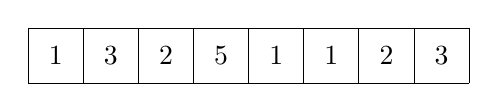
\begin{tikzpicture}[scale=0.7]
\draw (0,0) grid (8,1);

\node at (0.5,0.5) {$1$};
\node at (1.5,0.5) {$3$};
\node at (2.5,0.5) {$2$};
\node at (3.5,0.5) {$5$};
\node at (4.5,0.5) {$1$};
\node at (5.5,0.5) {$1$};
\node at (6.5,0.5) {$2$};
\node at (7.5,0.5) {$3$};
\end{tikzpicture}
\end{center}
例えば以下のように和が$8$となる連続部分配列があります。
\begin{center}
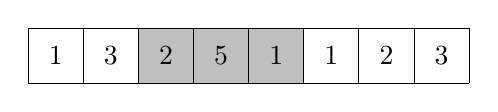
\begin{tikzpicture}[scale=0.7]
\fill[color=lightgray] (2,0) rectangle (5,1);
\draw (0,0) grid (8,1);

\node at (0.5,0.5) {$1$};
\node at (1.5,0.5) {$3$};
\node at (2.5,0.5) {$2$};
\node at (3.5,0.5) {$5$};
\node at (4.5,0.5) {$1$};
\node at (5.5,0.5) {$1$};
\node at (6.5,0.5) {$2$};
\node at (7.5,0.5) {$3$};
\end{tikzpicture}
\end{center}

この問題は2ポインターを使うことで$O(n)$時間で解くことができます。
これは、部分配列の最初と最後の場所を指すポインタを保持し、
各ステップで右ポインタを右にシフトしても和が$x$以下であるなら、ポインタを右にシフトします。
そうでなければ左ポインタを左にシフトします。
和がちょうど$x$になれば解が見つかったことになります。


ここで、$x=8$を達成するための操作を見てみます。
\begin{center}
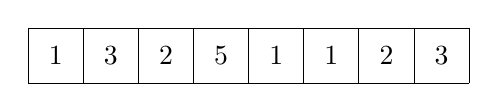
\begin{tikzpicture}[scale=0.7]
\draw (0,0) grid (8,1);

\node at (0.5,0.5) {$1$};
\node at (1.5,0.5) {$3$};
\node at (2.5,0.5) {$2$};
\node at (3.5,0.5) {$5$};
\node at (4.5,0.5) {$1$};
\node at (5.5,0.5) {$1$};
\node at (6.5,0.5) {$2$};
\node at (7.5,0.5) {$3$};
\end{tikzpicture}
\end{center}

まず、いくつか右ポインタを進め、
1, 3, 2まで進めると和は6です。

\begin{center}
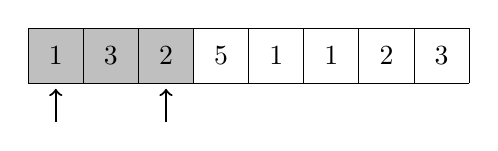
\begin{tikzpicture}[scale=0.7]
\fill[color=lightgray] (0,0) rectangle (3,1);
\draw (0,0) grid (8,1);

\node at (0.5,0.5) {$1$};
\node at (1.5,0.5) {$3$};
\node at (2.5,0.5) {$2$};
\node at (3.5,0.5) {$5$};
\node at (4.5,0.5) {$1$};
\node at (5.5,0.5) {$1$};
\node at (6.5,0.5) {$2$};
\node at (7.5,0.5) {$3$};

\draw[thick,->] (0.5,-0.7) -- (0.5,-0.1);
\draw[thick,->] (2.5,-0.7) -- (2.5,-0.1);
\end{tikzpicture}
\end{center}

さらに右のポインタを進めると$x$を超えてしまうので、
左のポインタを右に動かすことにします。

\begin{center}
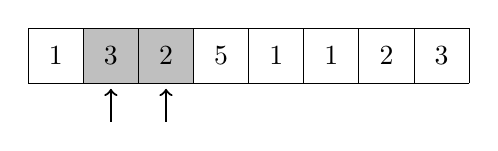
\begin{tikzpicture}[scale=0.7]
\fill[color=lightgray] (1,0) rectangle (3,1);
\draw (0,0) grid (8,1);

\node at (0.5,0.5) {$1$};
\node at (1.5,0.5) {$3$};
\node at (2.5,0.5) {$2$};
\node at (3.5,0.5) {$5$};
\node at (4.5,0.5) {$1$};
\node at (5.5,0.5) {$1$};
\node at (6.5,0.5) {$2$};
\node at (7.5,0.5) {$3$};

\draw[thick,->] (1.5,-0.7) -- (1.5,-0.1);
\draw[thick,->] (2.5,-0.7) -- (2.5,-0.1);
\end{tikzpicture}
\end{center}

この状態でも5を加えると$x$を超えてしまうので、左のポインタをもう1つ右に進めます。
これで右のポインタを右に進められることになり$2+5+1=8$となって$x$を見つけることができました。

\begin{center}
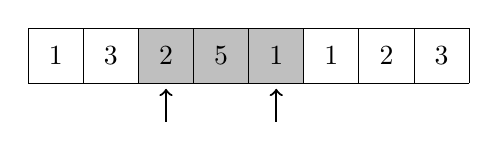
\begin{tikzpicture}[scale=0.7]
\fill[color=lightgray] (2,0) rectangle (5,1);
\draw (0,0) grid (8,1);

\node at (0.5,0.5) {$1$};
\node at (1.5,0.5) {$3$};
\node at (2.5,0.5) {$2$};
\node at (3.5,0.5) {$5$};
\node at (4.5,0.5) {$1$};
\node at (5.5,0.5) {$1$};
\node at (6.5,0.5) {$2$};
\node at (7.5,0.5) {$3$};

\draw[thick,->] (2.5,-0.7) -- (2.5,-0.1);
\draw[thick,->] (4.5,-0.7) -- (4.5,-0.1);
\end{tikzpicture}
\end{center}

このアルゴリズムの実行時間の見積もりには右ポインタの移動ステップ数に注目しましょう。
ポインタが1回のターンで何ステップ動けるかというのは配列の値によって異なります。
ただしポインタは右にしか動かないので、アルゴリズム中に合計$O(n)$ステップしか動けないことに注目しましょう。
同様に左のポインタはアルゴリズム中に$O(n)$ステップ移動するのでアルゴリズム全体は$O(n)$で動作します。

\subsubsection{2SUM problem}

\index{2SUM問題 - 2SUM problem}

別の問題を考えましょう。$n$要素の配列と$x$が与えられたとき、
和が$x$となる配列の2つの要素見つけるか、そのような値は存在しないことを出力しなさい、という問題です。
これを効率的に解くには配列の値を昇順に並べ替えます。
次に、2つのポインタを用いて配列を繰り返し処理します。
左のポインタは最初の値から始まり、1ターンごとに1ステップ右へ移動させます。
右のポインタは最後の値から始まり、左と右の値の合計が最大で$x$になるまで常に左に移動します。
例えば、次のような配列で$x=12$であるケースを考えましょう。

\begin{center}
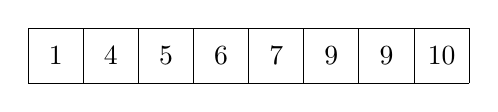
\begin{tikzpicture}[scale=0.7]
\draw (0,0) grid (8,1);

\node at (0.5,0.5) {$1$};
\node at (1.5,0.5) {$4$};
\node at (2.5,0.5) {$5$};
\node at (3.5,0.5) {$6$};
\node at (4.5,0.5) {$7$};
\node at (5.5,0.5) {$9$};
\node at (6.5,0.5) {$9$};
\node at (7.5,0.5) {$10$};
\end{tikzpicture}
\end{center}

ポインタの初期位置は以下の通りです。値の和は$1+10=11$で$x$より小さいです。

\begin{center}
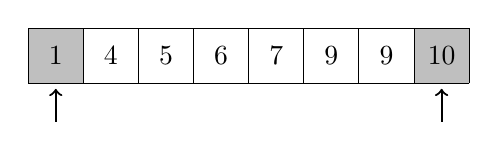
\begin{tikzpicture}[scale=0.7]
\fill[color=lightgray] (0,0) rectangle (1,1);
\fill[color=lightgray] (7,0) rectangle (8,1);
\draw (0,0) grid (8,1);

\node at (0.5,0.5) {$1$};
\node at (1.5,0.5) {$4$};
\node at (2.5,0.5) {$5$};
\node at (3.5,0.5) {$6$};
\node at (4.5,0.5) {$7$};
\node at (5.5,0.5) {$9$};
\node at (6.5,0.5) {$9$};
\node at (7.5,0.5) {$10$};

\draw[thick,->] (0.5,-0.7) -- (0.5,-0.1);
\draw[thick,->] (7.5,-0.7) -- (7.5,-0.1);
\end{tikzpicture}
\end{center}

そこで、左のポインタが右に1ステップ移動します。
ここで、右のポインターは左に3ステップ移動し、合計は$4 + 7 = 11$となる。

\begin{center}
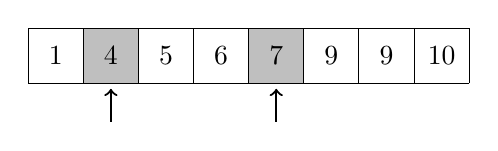
\begin{tikzpicture}[scale=0.7]
\fill[color=lightgray] (1,0) rectangle (2,1);
\fill[color=lightgray] (4,0) rectangle (5,1);
\draw (0,0) grid (8,1);

\node at (0.5,0.5) {$1$};
\node at (1.5,0.5) {$4$};
\node at (2.5,0.5) {$5$};
\node at (3.5,0.5) {$6$};
\node at (4.5,0.5) {$7$};
\node at (5.5,0.5) {$9$};
\node at (6.5,0.5) {$9$};
\node at (7.5,0.5) {$10$};

\draw[thick,->] (1.5,-0.7) -- (1.5,-0.1);
\draw[thick,->] (4.5,-0.7) -- (4.5,-0.1);
\end{tikzpicture}
\end{center}


左ポインタは再び右へ1ステップ移動します。
$5+7=12$という解が存在することが分かりました。

\begin{center}
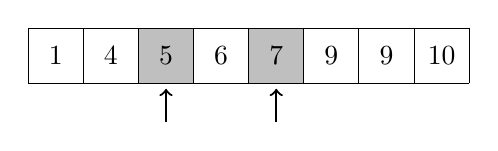
\begin{tikzpicture}[scale=0.7]
\fill[color=lightgray] (2,0) rectangle (3,1);
\fill[color=lightgray] (4,0) rectangle (5,1);
\draw (0,0) grid (8,1);

\node at (0.5,0.5) {$1$};
\node at (1.5,0.5) {$4$};
\node at (2.5,0.5) {$5$};
\node at (3.5,0.5) {$6$};
\node at (4.5,0.5) {$7$};
\node at (5.5,0.5) {$9$};
\node at (6.5,0.5) {$9$};
\node at (7.5,0.5) {$10$};

\draw[thick,->] (2.5,-0.7) -- (2.5,-0.1);
\draw[thick,->] (4.5,-0.7) -- (4.5,-0.1);
\end{tikzpicture}
\end{center}

実行時間を見積もります。まず、配列を$O(n \log n)$でソートし、次に両方のポインタを$O(n)$回移動させるため全体では$O(n \log n)$となります。
二分探索を用いれば、別の方法で$O(n \log n)$時間で解くこともできます。
配列の各値に対して和$x$となる値を二分探索すればよいです。

\index{3SUM problem}
これより難しい問題としては、和が$x$となる3つの配列値を求める\key{3SUM 問題} があります。
上記のアルゴリズムの考え方を用いると,この問題は に従って $O(n^2)$ 時間で解くことができます。
\footnote{長い間、3SUM 問題を $O(n^2)$ 時間より効率的に解くことは不可能と考えられていました。し
かし、2014 年に、そうではないことが判明した \cite{gro14} }.

\section{最も近い小さな要素 - Nearest smaller elements}

\index{最も近い小さな要素 - nearest smaller elements}

データ構造に対して行われた操作の回数を推定するために、
ならし解析がよく利用されます。演算の実行は入力によって不均等に分布するので、
アルゴリズムの特定のフェーズで演算が発生こととなりますが演算の総数には限りがあります。

ここで配列の各要素について既出の最も近い小さい要素,つまり配列内でその要素に先行する最初の小さい要素を見つける問題を考えてみます。
そのような要素が存在しないこともあり得ますが,その場合はアルゴリズムがそのことを報告するとしましょう。
まずは、この問題をスタック構造を用いてどのように効率的に解決できるかを見ていきます。

配列を左から右へ走査し,配列要素のスタックを維持します.
配列の各位置で,一番上の要素が現在の要素より小さくなるか,
スタックが空になるまで,スタックから要素を取り除いていきます.
そして,一番上の要素が現在の要素に最も近い小さい要素であることを報告します.
また,スタックが空であれば,そのような要素は存在しません.
そして、現在の要素をスタックに追加するといった操作を続けます。

例として、次のような配列を考えてみましょう。

\begin{center}
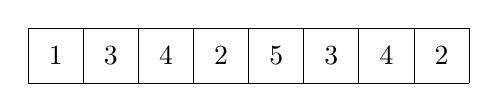
\begin{tikzpicture}[scale=0.7]
\draw (0,0) grid (8,1);

\node at (0.5,0.5) {$1$};
\node at (1.5,0.5) {$3$};
\node at (2.5,0.5) {$4$};
\node at (3.5,0.5) {$2$};
\node at (4.5,0.5) {$5$};
\node at (5.5,0.5) {$3$};
\node at (6.5,0.5) {$4$};
\node at (7.5,0.5) {$2$};
\end{tikzpicture}
\end{center}

まず、各要素が前の要素より大きいので、1、3、4の要素がスタックに追加されます。
したがって、4の最も近い小さい要素は3であり、3の最も近い小さい要素は1となります。
\begin{center}
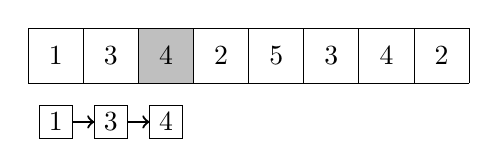
\begin{tikzpicture}[scale=0.7]
\fill[color=lightgray] (2,0) rectangle (3,1);
\draw (0,0) grid (8,1);

\node at (0.5,0.5) {$1$};
\node at (1.5,0.5) {$3$};
\node at (2.5,0.5) {$4$};
\node at (3.5,0.5) {$2$};
\node at (4.5,0.5) {$5$};
\node at (5.5,0.5) {$3$};
\node at (6.5,0.5) {$4$};
\node at (7.5,0.5) {$2$};

\draw (0.2,0.2-1.2) rectangle (0.8,0.8-1.2);
\draw (1.2,0.2-1.2) rectangle (1.8,0.8-1.2);
\draw (2.2,0.2-1.2) rectangle (2.8,0.8-1.2);

\node at (0.5,0.5-1.2) {$1$};
\node at (1.5,0.5-1.2) {$3$};
\node at (2.5,0.5-1.2) {$4$};

\draw[->,thick] (0.8,0.5-1.2) -- (1.2,0.5-1.2);
\draw[->,thick] (1.8,0.5-1.2) -- (2.2,0.5-1.2);
\end{tikzpicture}
\end{center}

次の要素である2は、スタックの一番上の2つの要素より小さい。
このため、要素 3 と 4 がスタックからpopし
次に要素 2 がスタックに追加されます。
その最も近い小さい要素は1となります。

\begin{center}
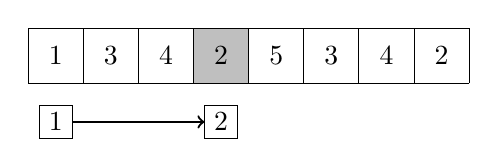
\begin{tikzpicture}[scale=0.7]
\fill[color=lightgray] (3,0) rectangle (4,1);
\draw (0,0) grid (8,1);

\node at (0.5,0.5) {$1$};
\node at (1.5,0.5) {$3$};
\node at (2.5,0.5) {$4$};
\node at (3.5,0.5) {$2$};
\node at (4.5,0.5) {$5$};
\node at (5.5,0.5) {$3$};
\node at (6.5,0.5) {$4$};
\node at (7.5,0.5) {$2$};

\draw (0.2,0.2-1.2) rectangle (0.8,0.8-1.2);
\draw (3.2,0.2-1.2) rectangle (3.8,0.8-1.2);

\node at (0.5,0.5-1.2) {$1$};
\node at (3.5,0.5-1.2) {$2$};

\draw[->,thick] (0.8,0.5-1.2) -- (3.2,0.5-1.2);
\end{tikzpicture}
\end{center}

そして、要素5は要素2より大きいのでスタックに追加され、その最も近い小さい要素は2となります。

\begin{center}
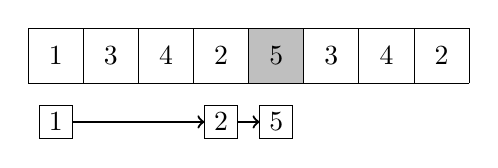
\begin{tikzpicture}[scale=0.7]
\fill[color=lightgray] (4,0) rectangle (5,1);
\draw (0,0) grid (8,1);

\node at (0.5,0.5) {$1$};
\node at (1.5,0.5) {$3$};
\node at (2.5,0.5) {$4$};
\node at (3.5,0.5) {$2$};
\node at (4.5,0.5) {$5$};
\node at (5.5,0.5) {$3$};
\node at (6.5,0.5) {$4$};
\node at (7.5,0.5) {$2$};

\draw (0.2,0.2-1.2) rectangle (0.8,0.8-1.2);
\draw (3.2,0.2-1.2) rectangle (3.8,0.8-1.2);
\draw (4.2,0.2-1.2) rectangle (4.8,0.8-1.2);

\node at (0.5,0.5-1.2) {$1$};
\node at (3.5,0.5-1.2) {$2$};
\node at (4.5,0.5-1.2) {$5$};

\draw[->,thick] (0.8,0.5-1.2) -- (3.2,0.5-1.2);
\draw[->,thick] (3.8,0.5-1.2) -- (4.2,0.5-1.2);
\end{tikzpicture}
\end{center}

この後、要素5をスタックから取り除き、要素3、4をスタックに追加しましょう。
\begin{center}
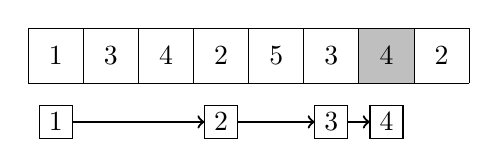
\begin{tikzpicture}[scale=0.7]
\fill[color=lightgray] (6,0) rectangle (7,1);
\draw (0,0) grid (8,1);

\node at (0.5,0.5) {$1$};
\node at (1.5,0.5) {$3$};
\node at (2.5,0.5) {$4$};
\node at (3.5,0.5) {$2$};
\node at (4.5,0.5) {$5$};
\node at (5.5,0.5) {$3$};
\node at (6.5,0.5) {$4$};
\node at (7.5,0.5) {$2$};

\draw (0.2,0.2-1.2) rectangle (0.8,0.8-1.2);
\draw (3.2,0.2-1.2) rectangle (3.8,0.8-1.2);
\draw (5.2,0.2-1.2) rectangle (5.8,0.8-1.2);
\draw (6.2,0.2-1.2) rectangle (6.8,0.8-1.2);

\node at (0.5,0.5-1.2) {$1$};
\node at (3.5,0.5-1.2) {$2$};
\node at (5.5,0.5-1.2) {$3$};
\node at (6.5,0.5-1.2) {$4$};

\draw[->,thick] (0.8,0.5-1.2) -- (3.2,0.5-1.2);
\draw[->,thick] (3.8,0.5-1.2) -- (5.2,0.5-1.2);
\draw[->,thick] (5.8,0.5-1.2) -- (6.2,0.5-1.2);
\end{tikzpicture}
\end{center}

最後に、1以外のすべての要素がスタックから取り除かれ、最後の要素2がスタックに追加されます。
\begin{center}
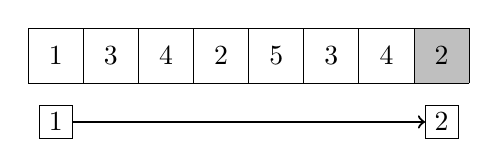
\begin{tikzpicture}[scale=0.7]
\fill[color=lightgray] (7,0) rectangle (8,1);
\draw (0,0) grid (8,1);

\node at (0.5,0.5) {$1$};
\node at (1.5,0.5) {$3$};
\node at (2.5,0.5) {$4$};
\node at (3.5,0.5) {$2$};
\node at (4.5,0.5) {$5$};
\node at (5.5,0.5) {$3$};
\node at (6.5,0.5) {$4$};
\node at (7.5,0.5) {$2$};

\draw (0.2,0.2-1.2) rectangle (0.8,0.8-1.2);
\draw (7.2,0.2-1.2) rectangle (7.8,0.8-1.2);

\node at (0.5,0.5-1.2) {$1$};
\node at (7.5,0.5-1.2) {$2$};

\draw[->,thick] (0.8,0.5-1.2) -- (7.2,0.5-1.2);
\end{tikzpicture}
\end{center}

アルゴリズムは入力によるスタックオペレーションの総数に依存します。
現在の要素がスタックの一番上の要素より大きい場合、直接スタックに追加され効率的です。
ところが、スタックにいくつかの大きな要素が含まれることがあり、それらを取り除くのに時間がかかるように思えます。
ですが、ここで注目すべきなのは各要素はスタックに最大一回追加され最大一回削除されるという点です。
つまり、各要素は $O(1)$ スタック操作を引き起こすのでアルゴリズムは $O(n)$ 時間で動作するといえます。

\section{最小スライディングウィンドウ - Sliding window minimum}

\index{スライディングウィンドウ - sliding window}
\index{最小スライディングウィンドウ - sliding window minimum}

\key{スライディングウィンドウ - sliding window}は、
配列の左から右へ移動する一定サイズの部分配列のことです。
各ウィンドウの位置で、窓の中の要素について何らかの情報を計算します。
ここでは、\key{最小スライディングウィンドウ - sliding window minimum}を維持する問題、
つまり、各ウィンドウ内の最小値を報告することに焦点を当てます。

スライディングウィンドウの最小値は、
前述の最も近い小さい要素を計算するのに用いたのと同様の考え方で計算することができます。
各要素が前の要素より大きい待ち行列を維持し、
最初の要素は常に窓の内側の最小要素に対応するようにします。
各ウィンドウの移動後、最後のキューの要素が新しいウィンドウの要素より小さくなるか、
キューが空になるまで、キューの末尾から要素を削除していきます。
また、最初の待ち行列の要素がもうウィンドウの中にない場合は、
それを削除します。最後に、新しいウィンドウの要素を待ち行列の最後に追加します。
例として、次のような配列を考えてみましょう。

\begin{center}
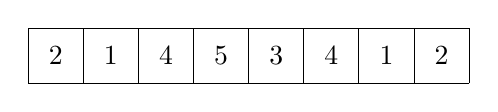
\begin{tikzpicture}[scale=0.7]
\draw (0,0) grid (8,1);

\node at (0.5,0.5) {$2$};
\node at (1.5,0.5) {$1$};
\node at (2.5,0.5) {$4$};
\node at (3.5,0.5) {$5$};
\node at (4.5,0.5) {$3$};
\node at (5.5,0.5) {$4$};
\node at (6.5,0.5) {$1$};
\node at (7.5,0.5) {$2$};
\end{tikzpicture}
\end{center}

スライディングウィンドウの大きさを4とすると、最初のウィンドウの位置で最小の値は1です。

\begin{center}
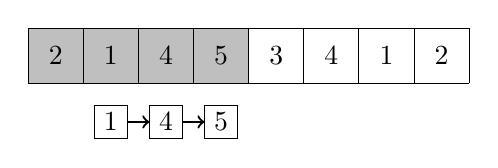
\begin{tikzpicture}[scale=0.7]
\fill[color=lightgray] (0,0) rectangle (4,1);
\draw (0,0) grid (8,1);

\node at (0.5,0.5) {$2$};
\node at (1.5,0.5) {$1$};
\node at (2.5,0.5) {$4$};
\node at (3.5,0.5) {$5$};
\node at (4.5,0.5) {$3$};
\node at (5.5,0.5) {$4$};
\node at (6.5,0.5) {$1$};
\node at (7.5,0.5) {$2$};

\draw (1.2,0.2-1.2) rectangle (1.8,0.8-1.2);
\draw (2.2,0.2-1.2) rectangle (2.8,0.8-1.2);
\draw (3.2,0.2-1.2) rectangle (3.8,0.8-1.2);

\node at (1.5,0.5-1.2) {$1$};
\node at (2.5,0.5-1.2) {$4$};
\node at (3.5,0.5-1.2) {$5$};

\draw[->,thick] (1.8,0.5-1.2) -- (2.2,0.5-1.2);
\draw[->,thick] (2.8,0.5-1.2) -- (3.2,0.5-1.2);
\end{tikzpicture}
\end{center}

まず、ウィンドウは1ステップ右に移動します。
新しい要素3は待ち行列の要素4と5より小さいので、
要素4と5は待ち行列から取り除かれ、
要素3が待ち行列に追加されます。
最小の値はまだ1のままです。

\begin{center}
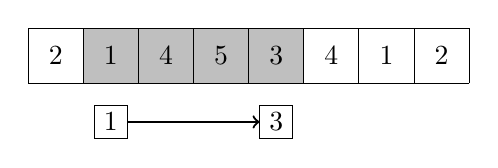
\begin{tikzpicture}[scale=0.7]
\fill[color=lightgray] (1,0) rectangle (5,1);
\draw (0,0) grid (8,1);

\node at (0.5,0.5) {$2$};
\node at (1.5,0.5) {$1$};
\node at (2.5,0.5) {$4$};
\node at (3.5,0.5) {$5$};
\node at (4.5,0.5) {$3$};
\node at (5.5,0.5) {$4$};
\node at (6.5,0.5) {$1$};
\node at (7.5,0.5) {$2$};

\draw (1.2,0.2-1.2) rectangle (1.8,0.8-1.2);
\draw (4.2,0.2-1.2) rectangle (4.8,0.8-1.2);

\node at (1.5,0.5-1.2) {$1$};
\node at (4.5,0.5-1.2) {$3$};

\draw[->,thick] (1.8,0.5-1.2) -- (4.2,0.5-1.2);
\end{tikzpicture}
\end{center}

この後、再びウィンドウが移動し、最小の要素1はウィンドウに属さなくなります。
従って、これはキューから取り除かれ、最小の値は3になります。
そして、新しい要素4がキューに追加されます。

\begin{center}
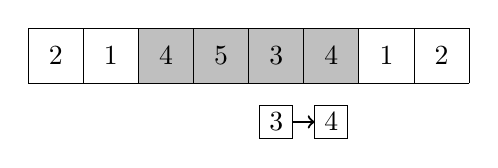
\begin{tikzpicture}[scale=0.7]
\fill[color=lightgray] (2,0) rectangle (6,1);
\draw (0,0) grid (8,1);

\node at (0.5,0.5) {$2$};
\node at (1.5,0.5) {$1$};
\node at (2.5,0.5) {$4$};
\node at (3.5,0.5) {$5$};
\node at (4.5,0.5) {$3$};
\node at (5.5,0.5) {$4$};
\node at (6.5,0.5) {$1$};
\node at (7.5,0.5) {$2$};

\draw (4.2,0.2-1.2) rectangle (4.8,0.8-1.2);
\draw (5.2,0.2-1.2) rectangle (5.8,0.8-1.2);

\node at (4.5,0.5-1.2) {$3$};
\node at (5.5,0.5-1.2) {$4$};

\draw[->,thick] (4.8,0.5-1.2) -- (5.2,0.5-1.2);
\end{tikzpicture}
\end{center}

次の新しい要素1は、待ち行列のすべての要素より小さいです。
このため、キューからすべての要素が削除され、要素1だけが含まれるようになります。

\begin{center}
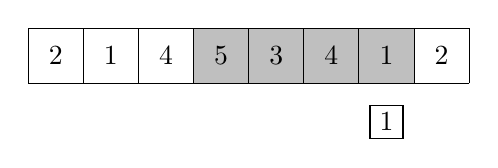
\begin{tikzpicture}[scale=0.7]
\fill[color=lightgray] (3,0) rectangle (7,1);
\draw (0,0) grid (8,1);

\node at (0.5,0.5) {$2$};
\node at (1.5,0.5) {$1$};
\node at (2.5,0.5) {$4$};
\node at (3.5,0.5) {$5$};
\node at (4.5,0.5) {$3$};
\node at (5.5,0.5) {$4$};
\node at (6.5,0.5) {$1$};
\node at (7.5,0.5) {$2$};

\draw (6.2,0.2-1.2) rectangle (6.8,0.8-1.2);

\node at (6.5,0.5-1.2) {$1$};
\end{tikzpicture}
\end{center}

最後に、ウィンドウは最後の位置に到達します。
要素2がキューに追加されるが、ウィンドウ内の最小値はまだ1のままです。

\begin{center}
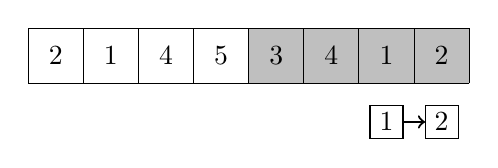
\begin{tikzpicture}[scale=0.7]
\fill[color=lightgray] (4,0) rectangle (8,1);
\draw (0,0) grid (8,1);

\node at (0.5,0.5) {$2$};
\node at (1.5,0.5) {$1$};
\node at (2.5,0.5) {$4$};
\node at (3.5,0.5) {$5$};
\node at (4.5,0.5) {$3$};
\node at (5.5,0.5) {$4$};
\node at (6.5,0.5) {$1$};
\node at (7.5,0.5) {$2$};

\draw (6.2,0.2-1.2) rectangle (6.8,0.8-1.2);
\draw (7.2,0.2-1.2) rectangle (7.8,0.8-1.2);

\node at (6.5,0.5-1.2) {$1$};
\node at (7.5,0.5-1.2) {$2$};

\draw[->,thick] (6.8,0.5-1.2) -- (7.2,0.5-1.2);
\end{tikzpicture}
\end{center}

各配列要素は正確に一度だけキューに追加され、最大一度だけキューから削除されるので、このアルゴリズムは$O(n)$時間で動作します。
